\documentclass{a0poster}
\usepackage{geometry}
\geometry{paper=a0paper}
\geometry{hmarginratio=1:1}
\geometry{vmarginratio=1:1}
\geometry{hmargin=25mm}
\geometry{vmargin=25mm}
\usepackage[pdftex]{graphicx}
%\usepackage{curves}
%\usepackage{algorithmic}
\usepackage[utf8]{inputenc}
\usepackage{amsmath}
\usepackage{amssymb}
\usepackage{amsthm}
%\usepackage{color, graphicx}
\usepackage{lipsum}
\usepackage{multicol}
\usepackage{subfigure}
%\usepackage{textpos}
\usepackage{url}
\usepackage{xcolor}
\usepackage{rotating}

\usepackage{mathptmx}
\usepackage[scaled=.90]{helvet}
\usepackage{courier}

%paket från kex
%\usepackage[T1]{fontenc}
%\usepackage{textcomp}
%\usepackage{lmodern}
\usepackage[swedish, english]{babel} 
%\usepackage[pdftex]{graphicx}
%\usepackage{wrapfig}
%\usepackage{float}
%\usepackage{cite}
%\usepackage{subfigure}
%%% define new commands %%%

\DeclareMathOperator{\sgn}{sgn}
\DeclareMathOperator{\sign}{sign}
\DeclareMathOperator{\diag}{diag}
\DeclareMathOperator{\supp}{supp}
\DeclareMathOperator{\res}{res}
\DeclareMathOperator{\meas}{meas}

\def\tol{{\textsc{tol}}}
\providecommand{\D}[1]{\,\mathrm{d}#1}

\newcommand{\mysmall}{\small}
\newcommand{\mynormalsize}{\normalsize}
\newcommand{\myFontSize}{\large}
\newcommand{\myTitleFontSize}{\Huge}
\newcommand{\mySubTitleFontSize}{\Large}
\newcommand{\mySubSubTitleFontSize}{\small}
\newcommand{\setLineThickness}{\linethickness{4mm}}
\newcommand{\myrule}{\rule{\textwidth}{3pt}}

%%% set new tolerances %%%%

\renewcommand{\textfraction}{0.05}
\renewcommand{\topfraction}{0.95}
\renewcommand{\bottomfraction}{0.95}
\renewcommand{\floatpagefraction}{0.35}
\setcounter{totalnumber}{5}

%%% options for multcol
\setlength{\columnsep}{25mm}

%%% begin document %%%

\begin{document}

\begin{tabular}{ll}

	\begin{minipage}{425mm}

		{\Huge\bf Simulering av ljudvågor med tillämpning inom datorspel}\\[10mm]
		{\Large\bf Alexander Aurell, \;Daniel von Witting,\\[3mm]
		Kandidatexamensarbete vid Numerisk Analys, KTH} \\


		\vspace*{5mm}

Idag är vi väldigt vana vid realistiska 3D grafikmotorer i tv- och datorspel. Detta inkluderar interaktiva miljöer och objekt, som tillfredsställande simulerar verkligheten. Ljudet har däremot inte följt samma utveckling och det krävs i dagsläget omfattande ansträngningar för designers och programmerare för att åstadkomma en acceptabel ljudupplevelse. En av de stora svårigheterna är begränsningarna på beräkningstid och lagringsutrymme. En ljudsimulering i ett datorspel måste kunna göras i realtid om det ska vara praktiskt användbar. Tanken med detta kandidatexamensarbete är att studera hurvida det är möjligt att skapa en ljudmotor baserad på den linjära akustiska vågekvationen och därmed skapa en realism som både förhöjer upplevelsen och underlättar implementeringen.


	\end{minipage}

\end{tabular}

\vspace*{25mm}

\begin{minipage}{\linewidth}

	\begin{multicols*}{2}

		\section*{Bakgrund}

Det finns generellt sett två olika typer av metoder för att simulera ljud i datorspel idag\cite{funkhouser}. Det ena sättet är att använda numeriska lösningar av den akustiska vågekvationen, t.ex. finita element metoder, det andra är att högfrekvensapproximera ljudet hos mottagaren baserat på att följa strålgången från källa till mottagare. Det stora problemet är att all ljudsimulering, likt grafiksimulering, ska ske i realtid. Därför finns en tillåten beräkningstid som indirekt reglerar hur kostsam simuleringen får vara. Att simulera fenomen såsom reflektion, diffraktion eller håligheter under denna begränsning är en utmaning.\\* 
Den senaste forskningen har bland annat gått ut på att få ner beräkningstiden för strålgångsmetoder, samt utveckla nya strålgångsmetoder och utvidga dessa för att lösa metodens brister. En huvudsaklig anledning är att GPU:erna (Graphics Processing Unit) i dagens datorer gör liknande operationer för ljus och grafik. Därför kan mycket prestanda vinnas om man lyckas att effektivt använda delar av grafiksimuleringen till att samtidigt behandla ljudutbredningen\cite{sjoberg}. Detta gäller dock inte bara strålgång, utan samma typ av lösning skulle gynna andra metoder med sämre komplexitet. GPU:er kan utföra fler operationer parallellt än vad en CPU (Central Processing Unit) kan. Om man skulle kunna avlasta CPU:n, som är den processor som utför bland annat ljudsimuleringar, kan man tjäna mycket beräkningstid, speciellt i realtidsberäkningar\cite{CPUcoGPU}. GPU:ns parallella arbetssätt gör att den är lämplig för att utföra FFT, Fast Fourier Transform, en algorim som kan användas för snabb beräkning av linjära partiella differentialekvationer. Detta är våran motivering till studiet av ljudsimulering baserat på den linjära akustiska vågekvationen. Detta skulle ge oss en realistisk modell för ljud i datorspel.\\*
\newline
Den linjära akustiska vågekvationen beskriver utveklingen av partikelpositionen $u$ eller det akustiska trycket $\rho$ som funktion av positionen och tiden. Ekvationen lyder för positionen
\begin{equation}
u_{tt} - v^{2}\Delta u = f(x,y,z,t),
\end{equation}
där v är ljudhastigheten i det aktuella mediet och $f(x,y,z,t)$ är en ljudkälla.\\*
I datorspel så rör sig spelaren ofta igenom många rum och i ett rum är den akustiska vågekvationen approximativt linjär. Denna linjäritet ger möjligheten att superponera ljudkällor. När vi angriper vårt problem måste det bestämmas vilka randvillkor som skall väljas för väggarna i våra simulationer. Alla material är till en viss grad absorberande i den meningen att ljudvågen tappar energi när den träffar väggen. Skriver man vågekvationen i en dimension på operatorform
\begin{equation}
\left(\frac{\partial^{2}}{\partial t^{2}} - v^{2}\frac{\partial^{2}}{\partial x^{2}}\right)u = 0
\end{equation}
kan följande faktorisering göras
\begin{equation}
\left(\frac{\partial}{\partial t} - v\frac{\partial}{\partial x}\right)\left(\frac{\partial}{\partial t} + v\frac{\partial}{\partial x}\right)u = 0.
\end{equation}
Det visar sig att faktorerna är en endast högergående respektive en endast vänstergående våg. Detta utnyttjas för att skriva ett absorberande villkor som säger att om en vänstergående våg träffar randen kommer en skalad högergående våg att reflekteras
\begin{equation*}
u_{t} - vu_{x} = \alpha\left(u_{t} + vu_{x}\right) 
\end{equation*}
\begin{equation} \label{eq:abc}
\Rightarrow u_{t} - v\left(\frac{1 + \alpha}{1 - \alpha}\right)u_{x} = 0, \qquad \alpha \in [0,1).
\end{equation}
Reflektionsparametern $\alpha$ kontrollerar hur mycket vågen reflekteras.
Då $\alpha \rightarrow 0$ så fås $u_{t} - vu_{x} = 0$ d.v.s. perfekt absorberande randvillkor. Då $\alpha \rightarrow 1$ kommer $u_{x}$-termen dominera och då fås $u_{x} = 0$, det klassiska Neumannvillkoret som ger full reflektion.\\*
\newline
		
		\section*{Metod}
När en spelplan är given så delas denna in i domäner i form av rektanglar. De kan vara olika stora och ha olika mått. Detta illustreras i den övre delen av figur 1. 
\newline
\newline
\begin{minipage}{\linewidth}
  \begin{center}
    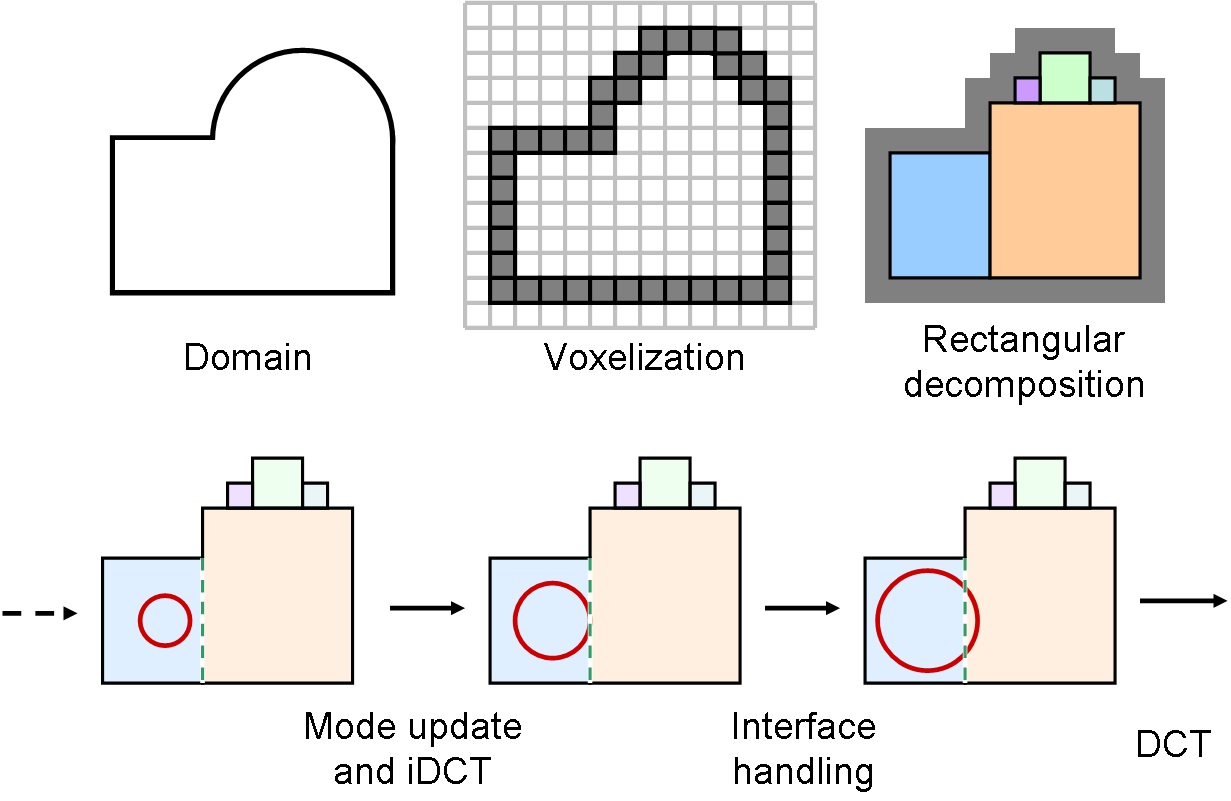
\includegraphics[width = 0.5\linewidth]{domain.jpg}\\*
    \caption{Figur 1. Domänen delas upp i rektanglar\cite{rect_decomp}.}\\*
  \end{center}
\end{minipage}
\newline
\newline
För att våran metod ska kunna behandla absorberande randvillkor spektralt måste vi först utveckla den för inhomogena randvillkor. Standardmetoden för att angripa inhomogena randvillkor är att dela upp vågfunktionen $u$,
\begin{equation}
u(x,t) = q(x,t) + w(x,t),
\end{equation}
där $q$ är en $[0,L]$-periodisk del som uppfyller vågekvationen med homogena randvillkor och en del $w$, känd för alla tider och positioner, som uppfyller de inhomogena randvillkoren. Nu kan vågekvationen skrivas upp för den periodiska delen $q$ med en källterm endast beroende utav $u$
\begin{equation} \label{eq:abcstep}
q_{tt} - v^{2}q_{xx} = \left(\frac{(L-x)^{2}}{2L}\right)(u_{t})_{xx}(0,t) - \left(\frac{x^{2}}{2L}\right)(u_{t})_{xx}(L,t) + \left(\frac{v^{2}}{L}\right)[u_{t}(L,t) - u_{t}(0,t)].
\end{equation}
Då $w$ är känt i varje steg och $q$ är periodisk över $[0,L]$ kan vi använda Discrete Cosine Transform för att uppdatera det inre av våra rektanglar.\\*
Sedan kommunicerar rektanglarna med varandra för att vågen skall kunna propagera mellan domänerna, illustrerat i den nedre delen av figur 1.


		
		\section*{Absorberande randvillkor}
%Ett numeriskt experiment i denna rapport går ut på att försöka implementera en absorberande rand till en domän [0,L] i en dimension. 

För att kontrollera det absorberande randvillkorets \eqref{eq:abc} realism görs följande numeriska experiment. Givet en domän [0,L] med randvillkoret \eqref{eq:abc} vid $x = 0$ och $x = L$ mäts vågens energi före och efter reflektion mot randen. Energin ska vara proportionell mot vågens amplitud i kvadrat, om vi halverar amplituden vid reflektion, $\alpha = 0.5$, så borde energin reduceras till en fjärdedel. I figur 2 presenteras resultatet av simuleringen med $\alpha = 0.5$. Simuleringen görs över en hel period T, alltså från initialläget tills vågen reflekterats och är tillbaka i startpositionen.\\*
\newline
\begin{minipage}{\linewidth}
\begin{tabular}{llll}
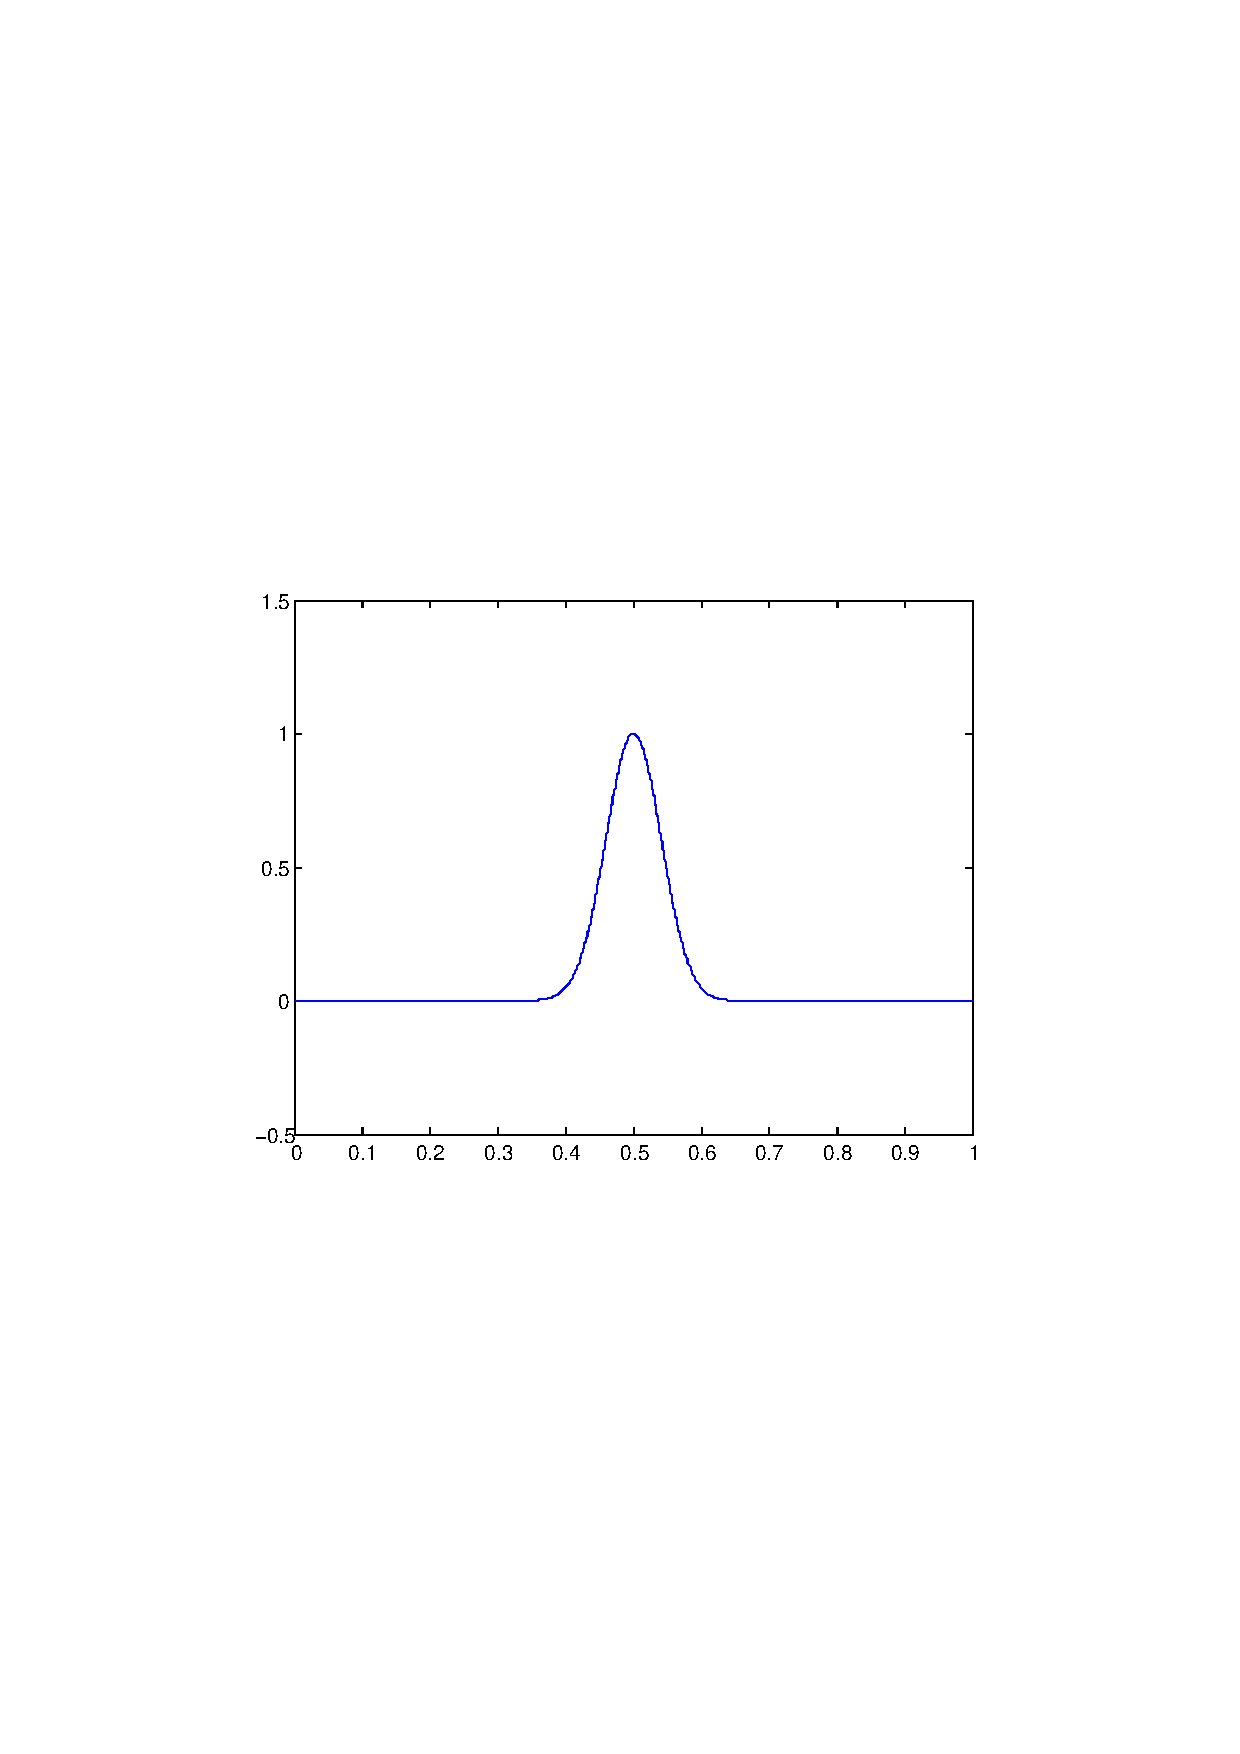
\includegraphics[trim = 5cm 10cm 4cm 10cm, width=.24\linewidth]{abc1.pdf} &
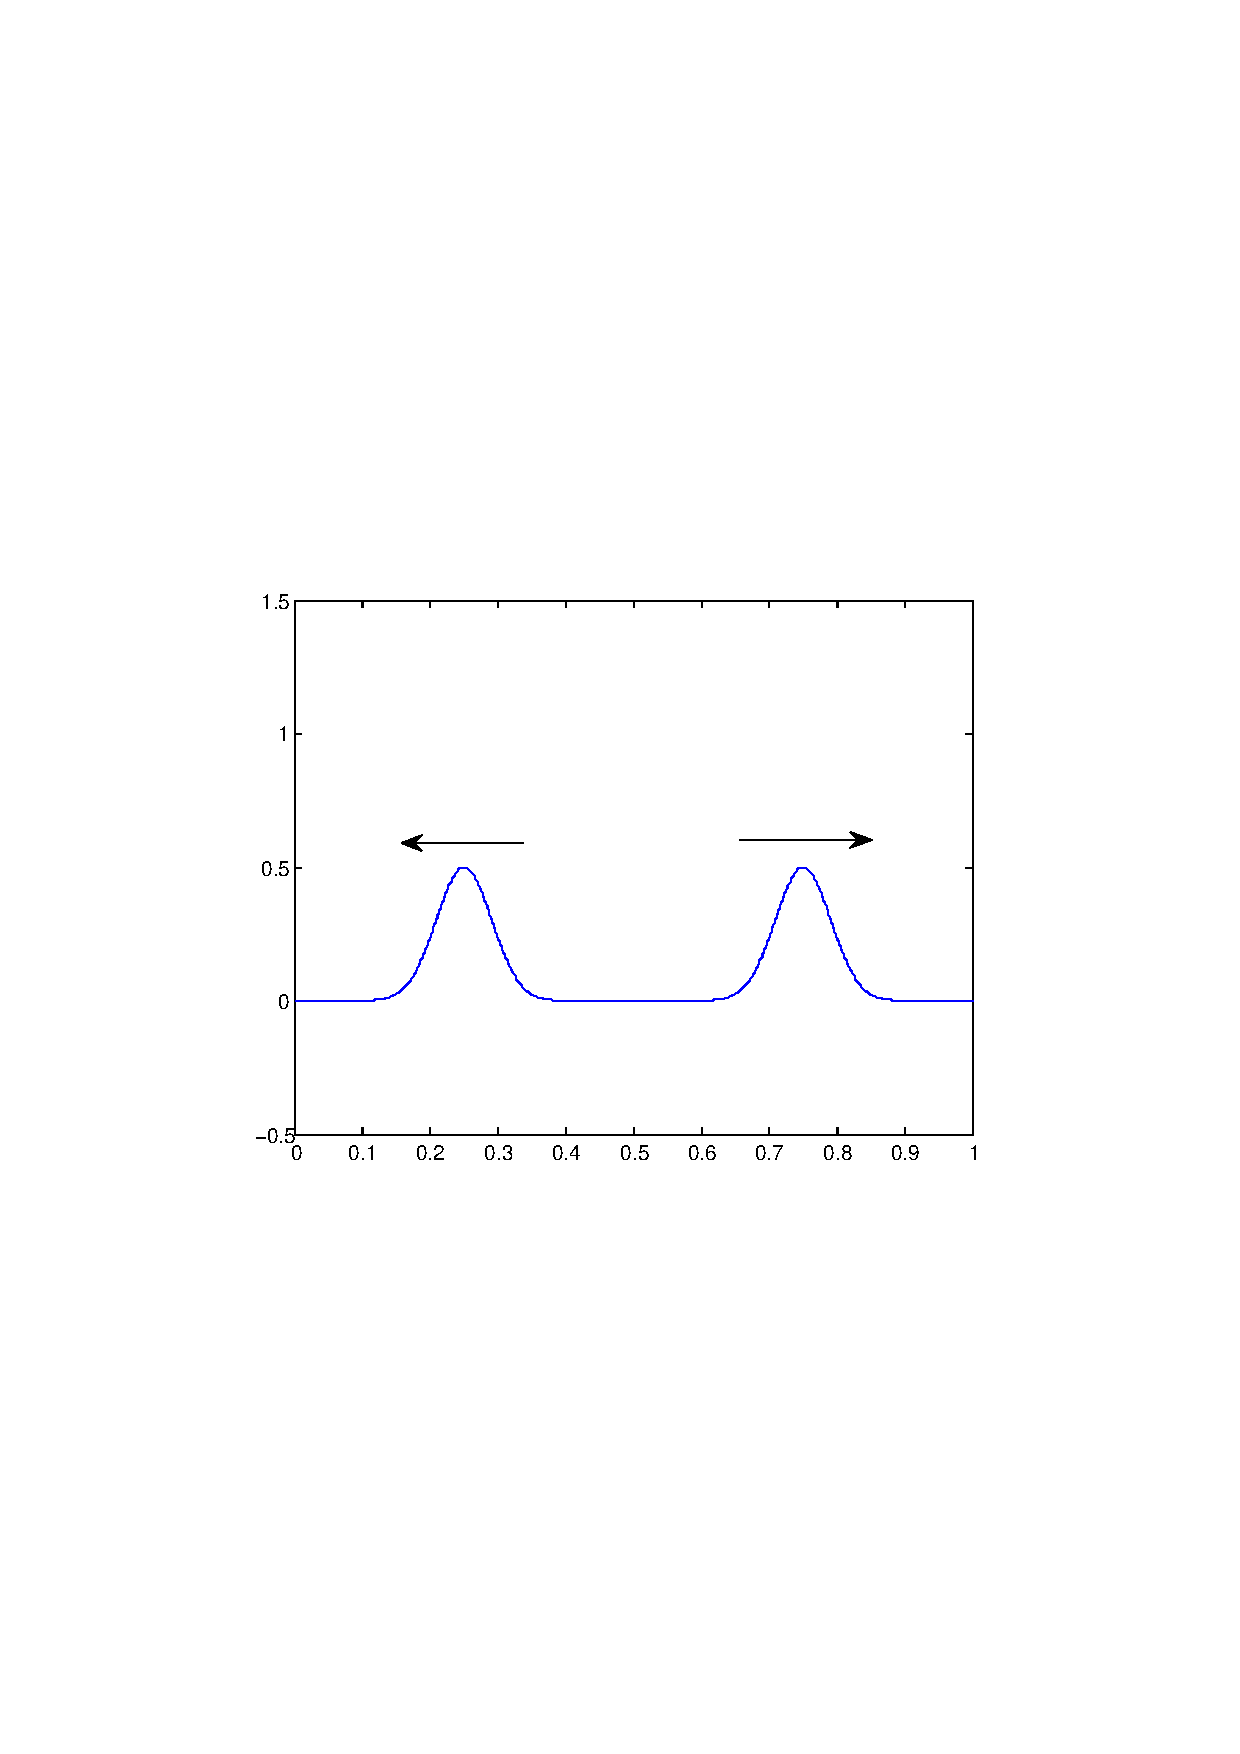
\includegraphics[trim = 5cm 10cm 4cm 10cm, width=.24\linewidth]{abc2.pdf} &
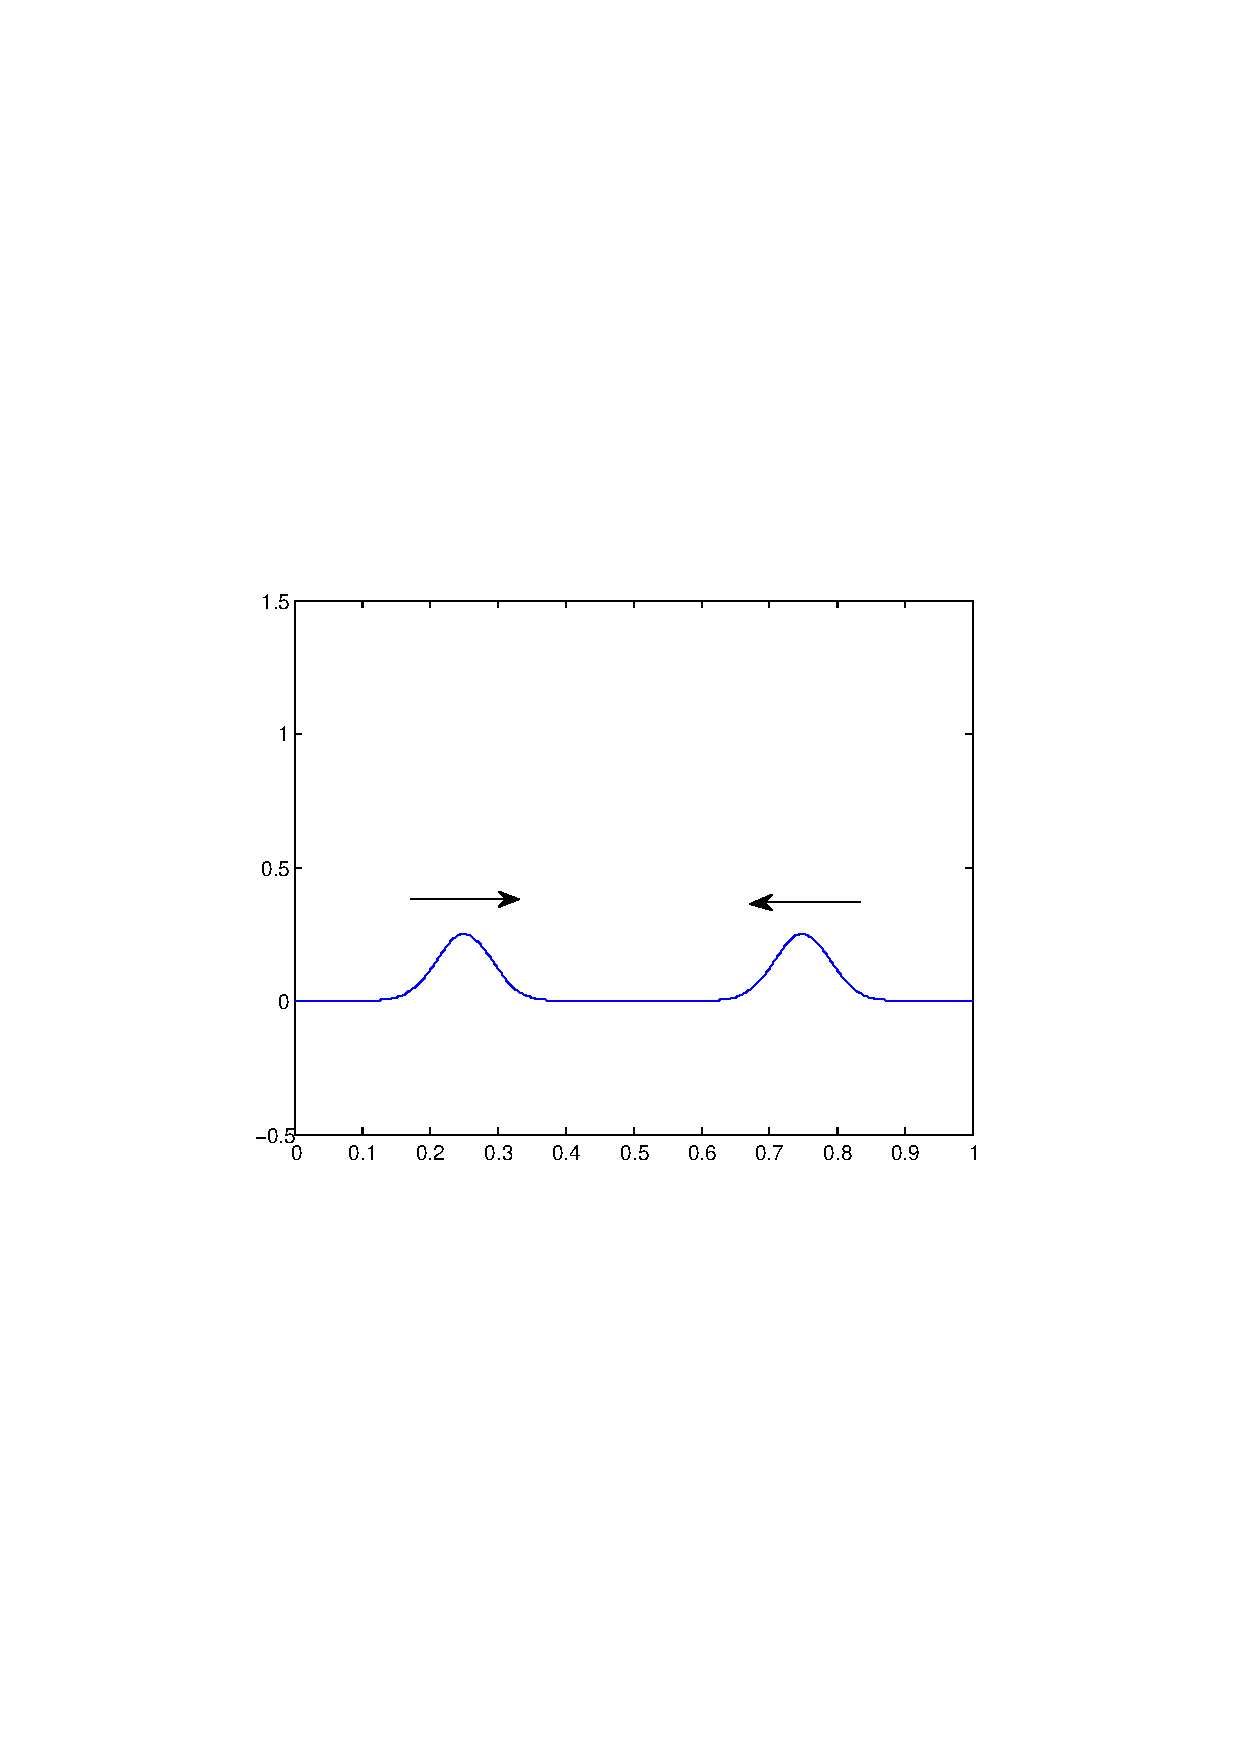
\includegraphics[trim = 5cm 10cm 4cm 10cm, width=.24\linewidth]{abc3.pdf} &
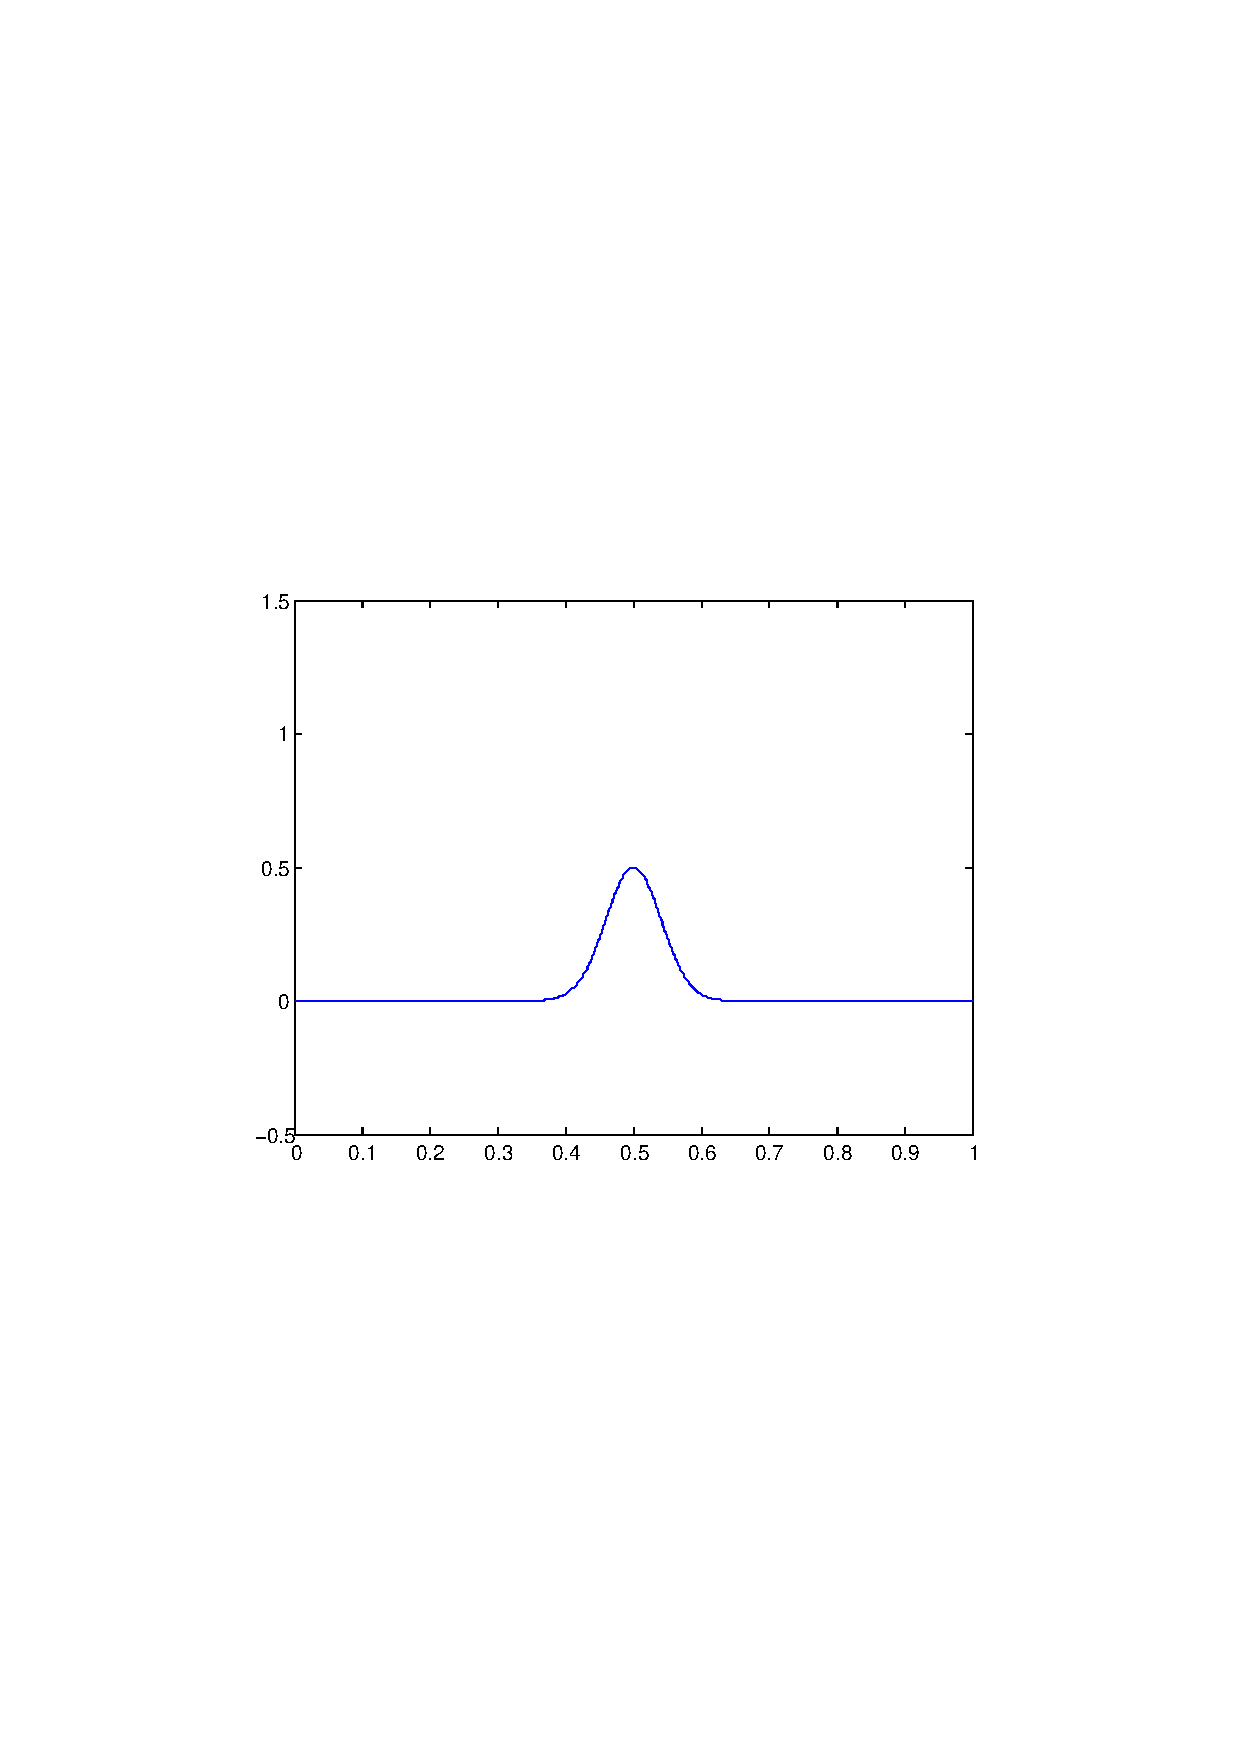
\includegraphics[trim = 5cm 10cm 4cm 10cm, width=.24\linewidth]{abc4.pdf}
\end{tabular}
\begin{center}
\caption{Figur 2. Från vänster ser vi vågen vid $t = 0$, $t = 0.25 T$, $t = 0.75 T$ och $t = T$.}\\*
\end{center}
\end{minipage}
\newline
\newline
Vågens energi mäts med en energiintegral härledd för Neumannvillkor. Denna ger ett inkorrekt resultat när vågen är nära randen, därför hämtas mätvärden när vågen helt lämnat randen. I tabell 1 kan det läsas av att medan amplituden har halverats så har energin minskat med en faktor fyra.\\*

\begin{minipage}{\linewidth}
	\begin{center}
    \begin{tabular}{| l | l | l | l |}
    \hline
    Tid & 0.25T &  0.75T \\ \hline
    Amplitud & 0.5 & 0.25 \\ \hline
    Energi & 10.8535 & 2.7136 \\ \hline
    \end{tabular}
    \end{center}
    \newline
    \begin{center}
    \caption{Tabell 1. Vågens amplitud och energi före och efter reflektion.}
    \end{center}
\end{minipage}


		
		\section*{Diffraktion}

Ljud har mycket längre våglängd än ljus vilket gör att ljudvågor inte beter sig likt synligt ljus när det stöter på ett hinder i sin väg utan sprids på grund av diffraktion. Diffraktionsgraden beror på förhållandet mellan vågens frekvens, som är omvänt proportionell mot våglängden, och hindrets dimensioner, ju lägre frekvens desto större hinder kan vågen komma runt. En metod baserad på strålgång ser förbi den här fysikaliska effekten. Vill en spelutvecklare ha diffraktion av ljud måste detta korrigeras för i efterhand. Flera ljudfenomen kan räknas upp som skapar liknande svårigheter i datorspel.\\*
\newline
Vi visar med detta numeriska experiment att diffraktion uppkommer utan någon extra ansträngning från våran metod, eftersom den är baserad på den linjära akustiska vågekvationen. En ljudkälla modelleras som en sinusfunktion just för att frekvensen då är lätt att kontrollera
\begin{equation}
f = \sin\left(\frac{n\pi}{K}\right),
\end{equation}
där $n$ är det aktuella tidssteget och $K$ är variabeln som styr frekvensen. Frekvensen hos $f$ är omvänt proportionell mot $K$.\\*
Vi placerar $f$ som en punktkälla i ett L-format rum så att en del av rummet inte kan ses från källan. I figur 3 ser vi rummet ovanifrån för fyra olika $K$ då tillräckligt lång tid har gått för att vågen ska ha spridit ut sig i hela rummet och stabiliserat sig runt hörnet. Vi ser att ju lägre frekvensen är desto mer diffraktion fås tills det saknas ljudskugga helt.\\*

\begin{minipage}{\linewidth}
\centering
\begin{tabular}{llll}
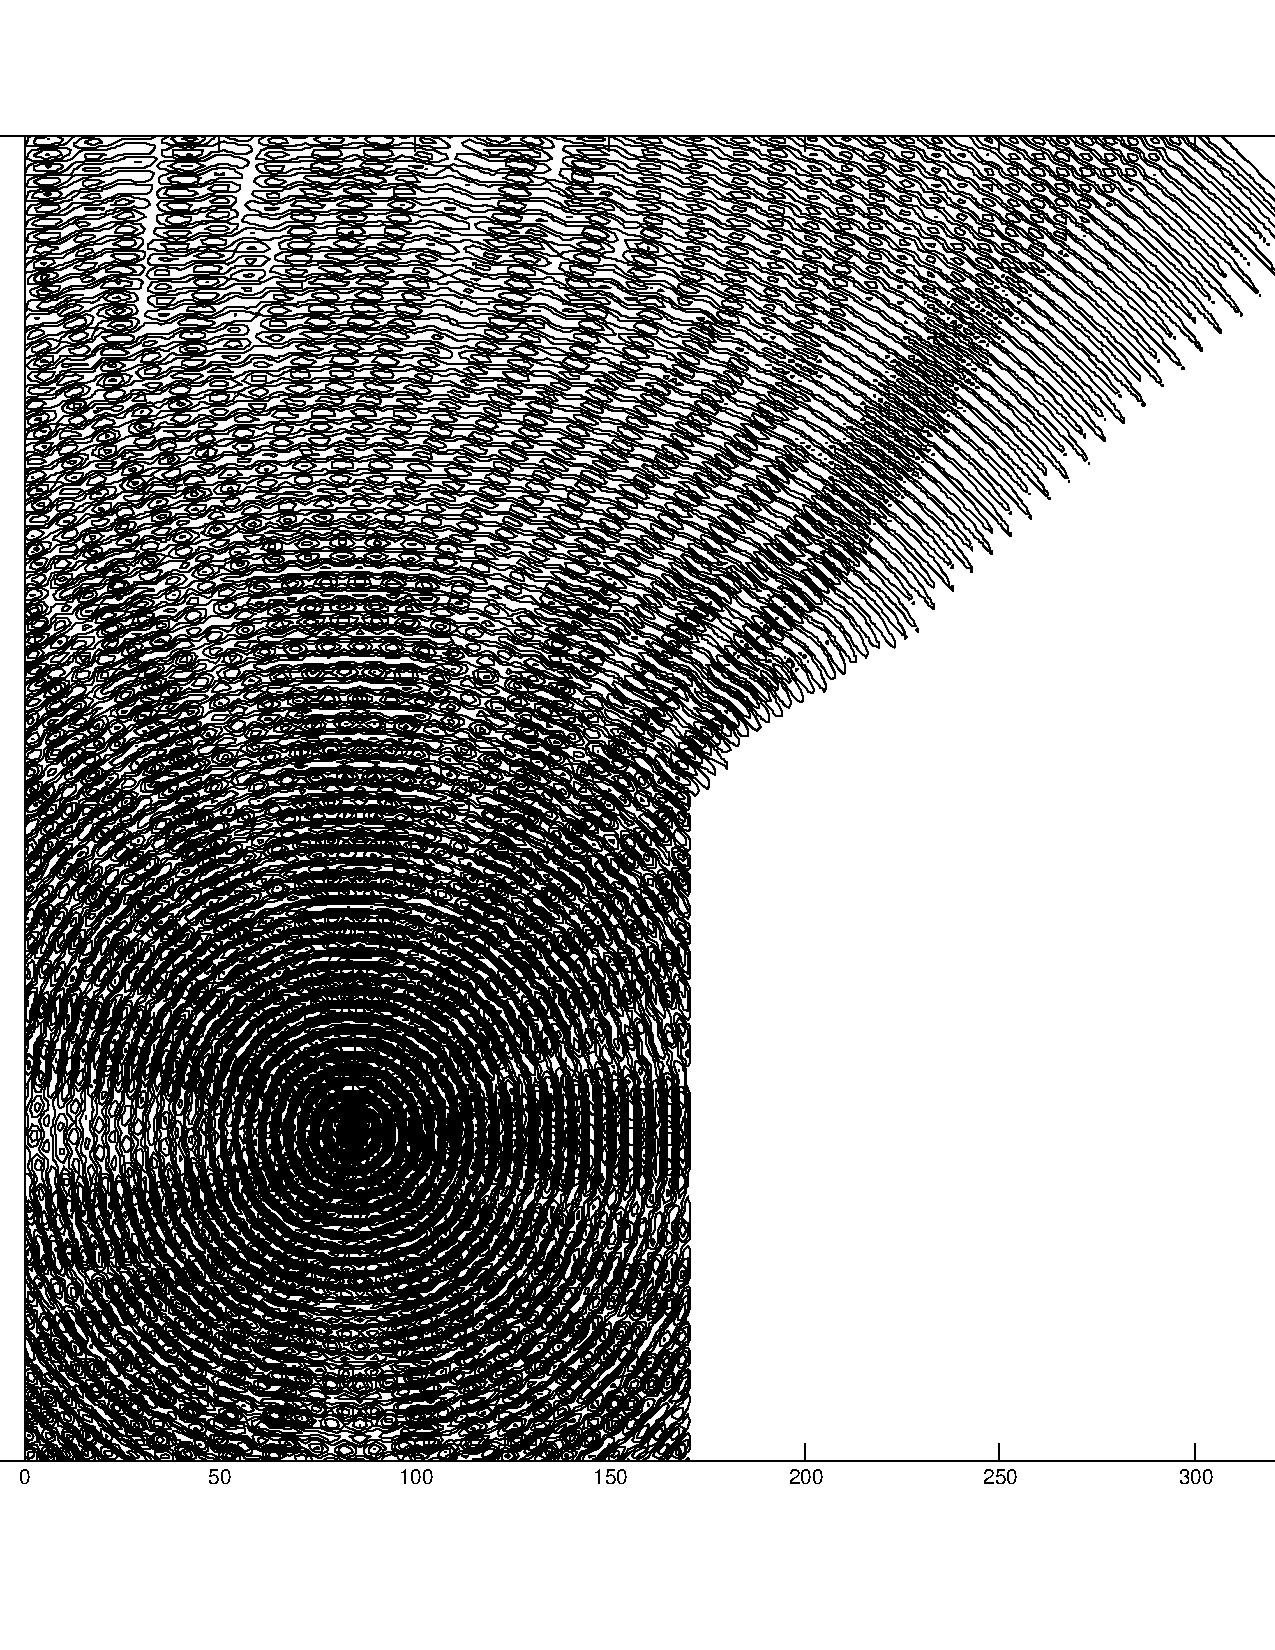
\includegraphics[width=.24\linewidth]{K_equals_5_bw.pdf} &
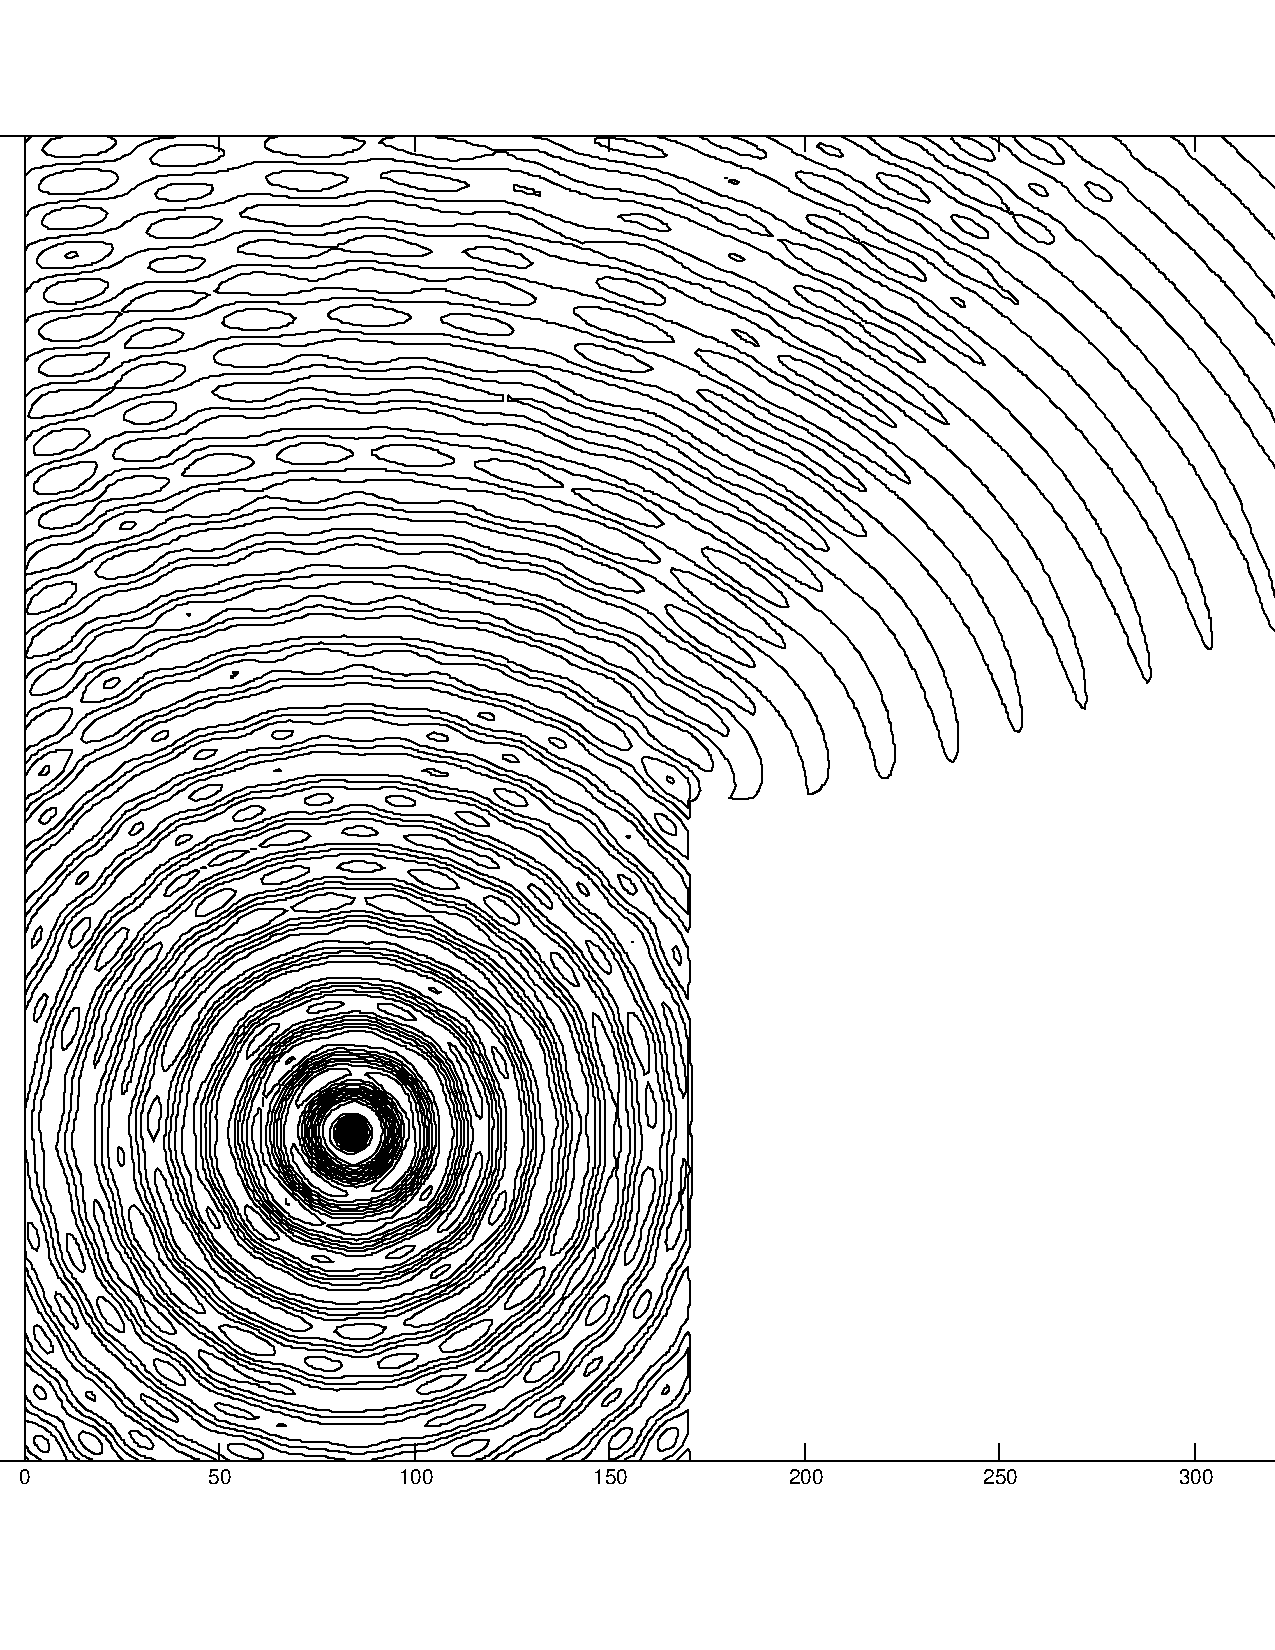
\includegraphics[width=.24\linewidth]{K_equals_13_bw.pdf} &
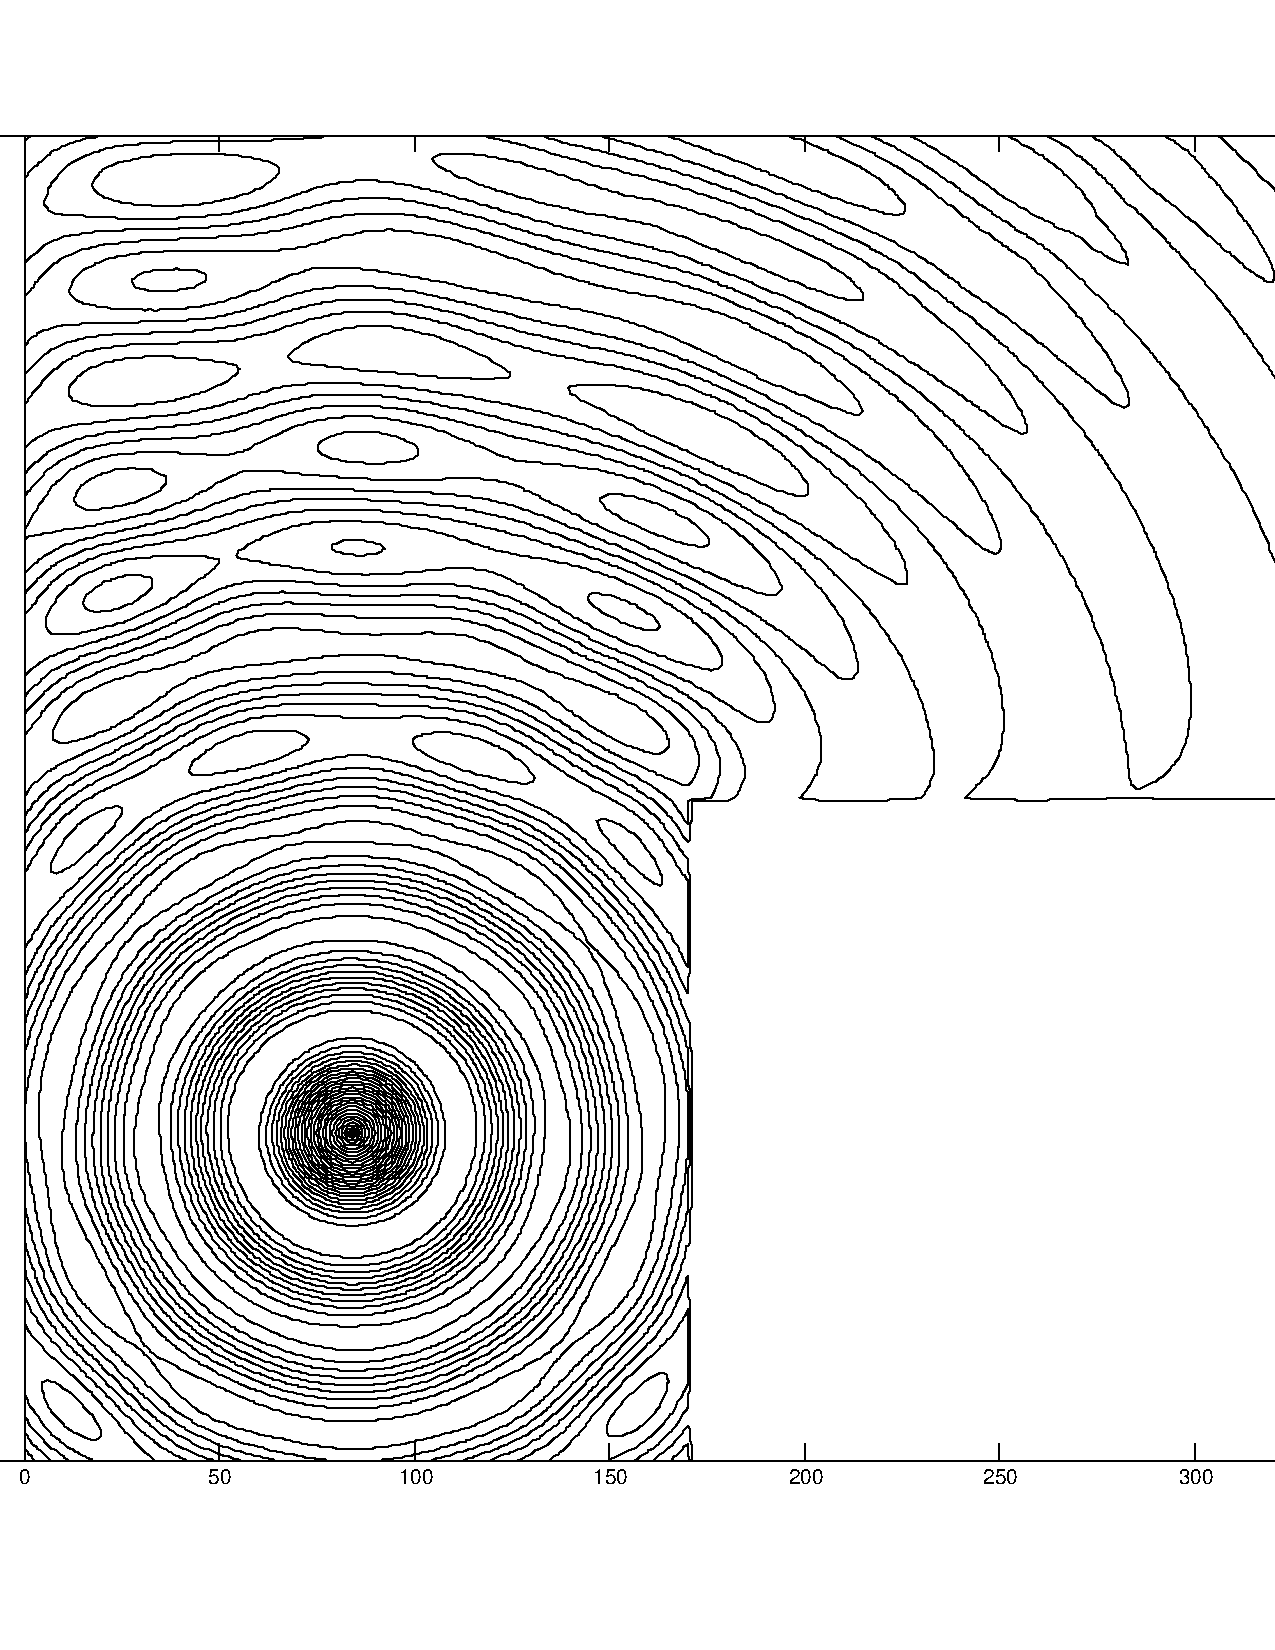
\includegraphics[width=.24\linewidth]{K_equals_36_bw.pdf} &
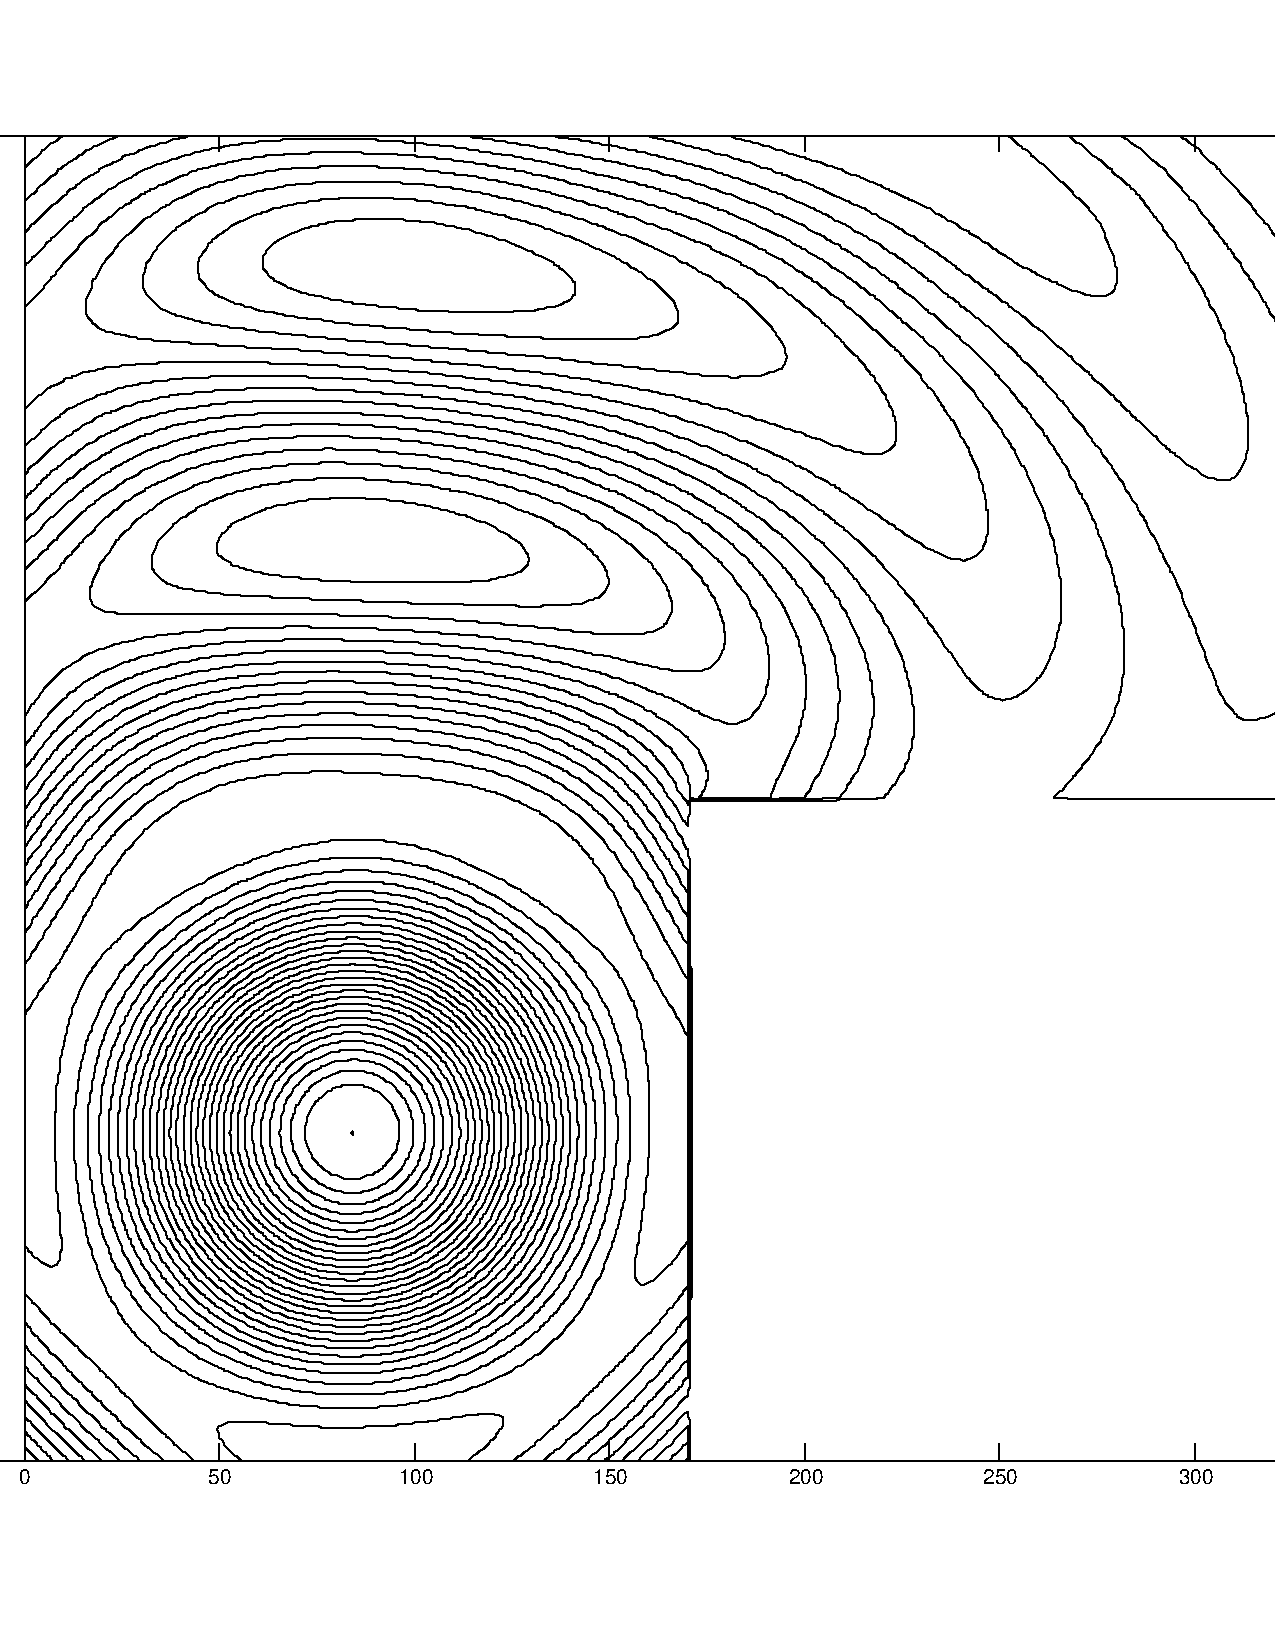
\includegraphics[width=.24\linewidth]{K_equals_100_bw.pdf}
\end{tabular}
\begin{center}
\caption{Figur 3. Från vänster: Diffraktion runt hörn med $K = 5$, $K = 13$, $K = 36$ och $K = 100$.}
\end{center}
\end{minipage}
		

		\bibliographystyle{vancouver}
		\bibliography{a0poster}

	\end{multicols*}

\end{minipage}


\end{document}
